\section{Performances}
\label{AABB_tree_section_performances}

We provide some performance numbers for the case where the AABB tree contains a set of polyhedron triangle facets. We measure both the tree construction time and the number of queries per second for a variety of intersection and distance queries. The machine used is a PC running Windows XP64 with an Intel CPU Core2 Extreme clocked at 3.06 GHz with 4GB of RAM. The kernel used is \ccc{Simple_cartesian<double>} (the fastest in our experiments). The program has been compiled with Visual C++ 2005 compiler with the O2 option (maximize speed).

\subsection{Intersections}

The surface triangle mesh chosen for benchmarking intersections is the knot model (14,400 triangles) available in the demo data folder. We measure the tree construction time for this model as well as for three denser versions subdivided through the Loop subdivision scheme which increases the number of triangles by a factor of four.

\begin{tabular}{|l|c|}
  \hline
  Number of triangles & Construction (in ms)\\
  \hline
   14,400 &   156 \\
   57,600 &   328 \\
  230,400 & 1,141 \\
  921,600 & 4,813 \\
  \hline
\end{tabular}

The following table measures the number of intersection queries per second on the 14,400 triangle version of the knot mesh model for ray, line, segment and plane queries. Each ray query is generated by choosing a random source point within the bounding box of the mesh and a random vector. A line or segment query is generated by choosing two random points within the bounding box. A plane query is generated by picking a random point within the bounding box and a random normal vector. Note that a plane query generically intersects many triangles of the input surface mesh. This explains the low performance numbers for the intersection functions which enumerate all intersections.

\begin{tabular}{|l|r|r|r|r|}
  \hline
  Function                              &     Ray &    Line & Segment &   Plane \\
  \hline
  do\_intersect()                       & 164,182 & 171,862 & 177,007 & 217,287 \\
  number\_of\_intersected\_primitives() &  89,075 &  90,334 & 104,475 &  10,248 \\
  any\_intersection()                   & 163,657 & 169,989 & 183,011 & 220,203 \\
  all\_intersections()                  &  62,625 &  60,168 &  73,525 &   3,026 \\
  all\_intersected\_primitives()        &  83,992 &  85,347 &  97,258 &   6,273 \\
  \hline
\end{tabular}

Curve \ref{fig:AABB-tree-bench} plots the number of queries per second (here the \ccc{all_intersections} function with random segment queries) against the number of input triangles for the knot triangle surface mesh.

% benchs over knot model
\begin{center}
    \label{fig:AABB-tree-bench}
    \begin{ccTexOnly}
      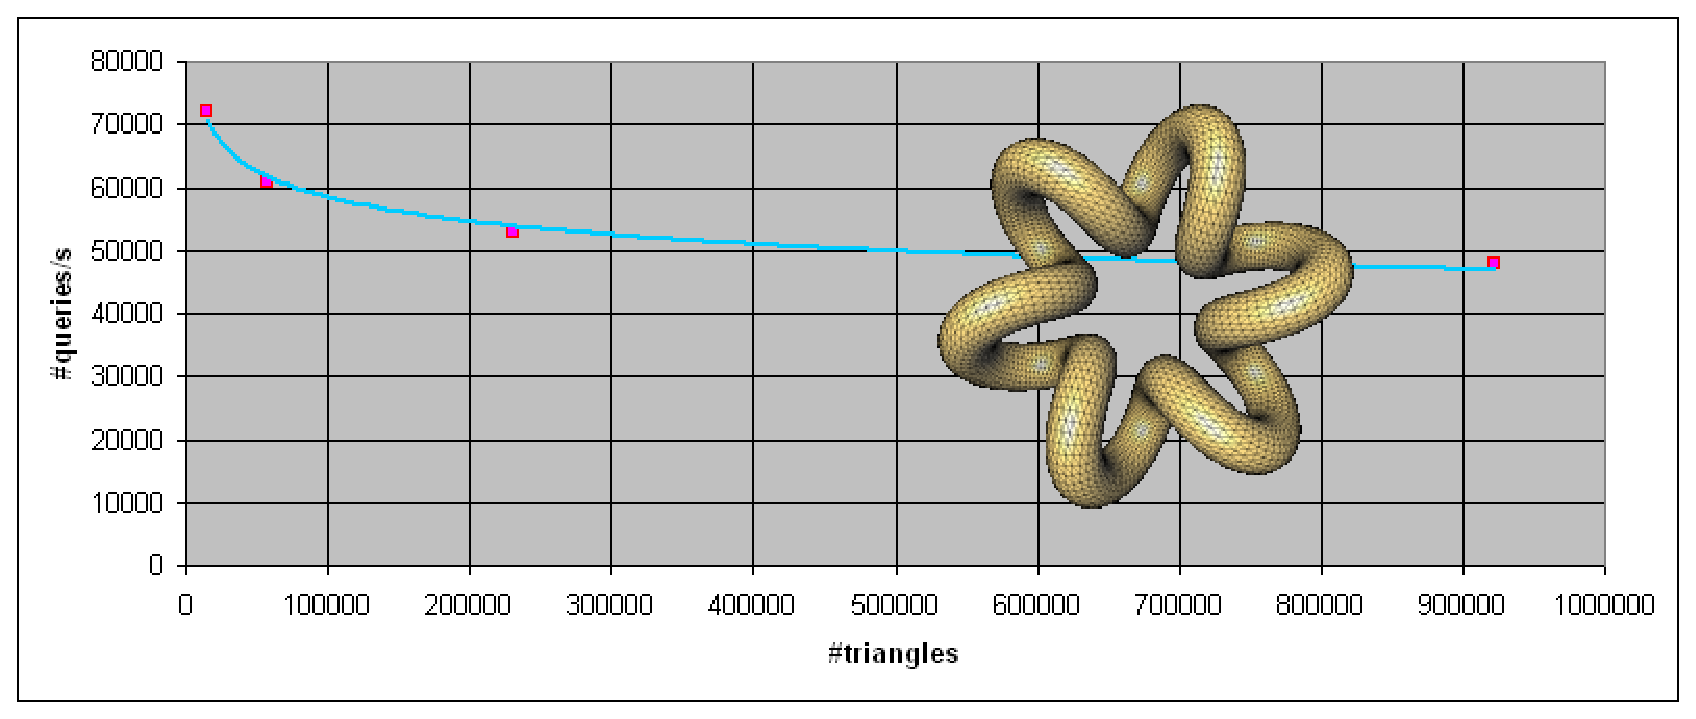
\includegraphics[width=1.0\textwidth]{AABB_tree/bench}
    \end{ccTexOnly}
    \begin{ccHtmlOnly}
        <img width="99%" border=0 src="./bench.png"><P>
    \end{ccHtmlOnly}
    \begin{figure}[h]
        \caption{Number of queries per second against number of triangles
                 for the knot model with 14K (shown), 57K, 230K and 921K
                 triangles. We call the \ccc{all_intersections} function
                 with segment queries randomly chosen within
                 the bounding box. }
    \end{figure}
\end{center}

\subsection{Distances}

The surface triangle mesh chosen for benchmarking distances is again the knot model in four increasing resolutions obtained through Loop subdivision. In the following table we first measure the tree construction time which includes the construction of the internal KD-tree data structure to accelerate the distance queries (note how the internal KD-tree construction is negligible compared to the AABB tree construction, while it brings an acceleration of up to one order of magnitude). We then measure the number of queries per second for the three types distance queries (\ccc{closest_point}, \ccc{squared_distance} and \ccc{closest_point_and_primitive}) from point queries randomly chosen inside the bounding box.

% TODO: redo with CGAL KD-tree issue fixed.

\begin{tabular}{|l|c|c|c|c|}
  \hline
  Nb triangles & Construction (in ms) & Closest\_point() & squared\_distance() & closest\_point\_and\_primitive() \\
  \hline
   14,400 &   157 & 31,472 & 33,529 & 34,817 \\
   57,600 &   330 & 15,602 & 16,355 & 17,106 \\
  230,400 & 1,203 &  6,528 &  8,287 &  8,683 \\
  921,600 & 5,047 &  4,399 &  4,221 &  4,424 \\
  \hline
\end{tabular}


\subsection{Memory}

The following curve plots the AABB tree memory consumption (without constructing the internal KD-tree) against the number of triangles of a polyhedron triangle surface mesh, when using the polyhedron triangle primitive. As expected the memory grows linearly and peaks to 128Mbytes for 2.3M triangles in the example shown. The AABB tree occupies approximately 60 bytes per primitive. 

% memory
\begin{center}
    \label{fig:AABB-tree-memory}
    \begin{ccTexOnly}
      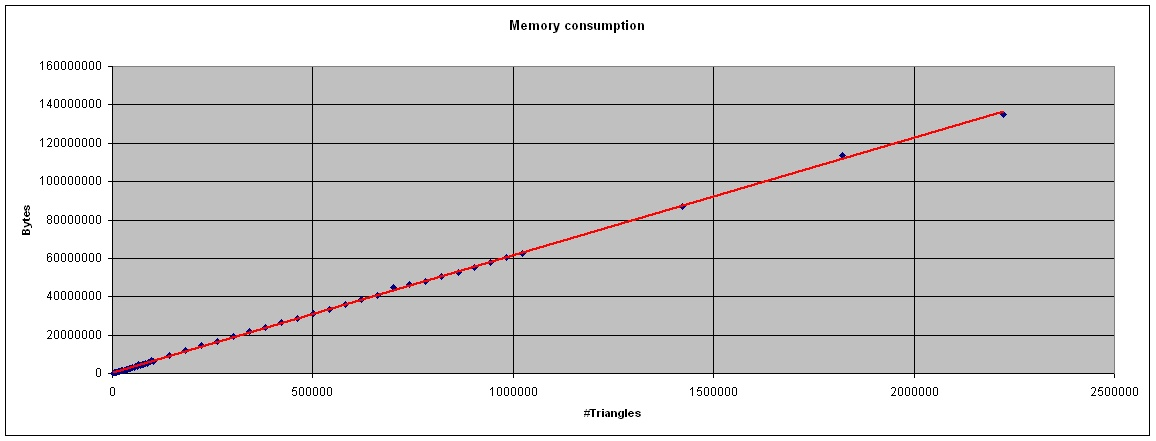
\includegraphics[width=1.0\textwidth]{AABB_tree/memory}
    \end{ccTexOnly}
    \begin{ccHtmlOnly}
        <img width="99%" border=0 src="./memory.png"><P>
    \end{ccHtmlOnly}
    \begin{figure}[h]
        \caption{Memory consumption in Bytes against number of triangles, here
                 ranging from 100 to 2.3M triangles.}
    \end{figure}
\end{center}

The memory consumption goes up to almost 100 bytes per primitive when constructing the internal KD-tree with one reference point per primitive (the default mode when calling the function \ccc{tree.accelerate_distance_queries()}). For large models we thus recommend to specify a lower number of reference point to construct the internal KD-tree through the same function which takes an iterator range as input.